%&tekstopmaak
\documentclass[../presentatie.tex]{subfiles}

%\addheadbox{section in head/foot}{\tiny\quad 1. Box}
%\addfootbox{structure}{\tiny\quad 2. Box}

%\setbeamercolor*{upper separation line head}{bg=red,fg=red}

%\makeatletter
%\setbeamertemplate{headline}
%{%
%%	\begin{beamercolorbox}{section in head/foot}
%%		\vskip2pt\insertnavigation{\paperwidth}\vskip2pt
%%		aaa
%%	\end{beamercolorbox}%
%  \begin{beamercolorbox}[colsep=1.5pt]{upper separation line head}
%\end{beamercolorbox}
%\begin{beamercolorbox}{section in head/foot}
%	\vskip2pt\insertnavigation{\paperwidth}\vskip2pt
%\end{beamercolorbox}%
%\ifbeamer@theme@subsection%
%\begin{beamercolorbox}[colsep=1.5pt]{middle separation line head}
%\end{beamercolorbox}
%\begin{beamercolorbox}[ht=2.5ex,dp=1.125ex,%
%	leftskip=.3cm,rightskip=.3cm plus1fil]{subsection in head/foot}
%	\usebeamerfont{subsection in head/foot}\insertsubsectionhead
%\end{beamercolorbox}%
%\fi%
%\begin{beamercolorbox}[colsep=1.5pt]{lower separation line head}
%\end{beamercolorbox}
%}
%\makeatother

\begin{document}
	\section{Tekstopmaak}
	\clearrecentlist
	
	%\subsection{Test}
	
	%\begin{frame}{$ \text{\LaTeX}\supset\text{Word} $}
	%	%\frametitle{$ \text{\LaTeX}\supset\text{Word} $}
	%	\begin{enumerate}
	%		\item Tekst vet / schuin
	%		\item Tekstgrootte
	%		\item Tekstkleur
	%		\item Lijntje
	%		\item Extra ruimte
	%		\item Kader
	%	\end{enumerate}
	%\end{frame}
	
	
	%\addtorecentlist{\hll|\\textbf|}
	\addtorecentlist{\textbf{\textbackslash textbf}}
	
	\begin{frame}
		\frametitle{Teksteffecten}
		
		\renewcommand{\arraystretch}{1.5}%
		\begin{tabularx}{0.5\textwidth}{ll}
			\toprule
			Resultaat {\global\showcount=1\relax}& Code\\
			\midrule
			\showlatex{\textbf{Tekst}}{\\textbf\{Tekst\}}\\
			\showlatex{\textit{Tekst}}{\\textit\{Tekst\}}\\
			\showlatex{\textsc{Tekst}}{\\textsc\{Tekst\}}\\
			\showlatex{\underline{Tekst}}{\\underline\{Tekst\}}\\
			%\showlatex{\large{Tekst}}{\\large\{Tekst\}}\\
			\bottomrule
		\end{tabularx}%
		\begin{tabularx}{0.5\textwidth}{ll}
			\toprule
			Resultaat {\global\showcount=5\relax}& Code\\
			\midrule
			\showlatex{\texttt{Tekst}}{\\texttt\{Tekst\}}\\
			%\showlatex{\textsl{Tekst}}{\\textsl\{Tekst\}}\\
			\showlatex{{\tiny Tekst}}{\{\\tiny Tekst\}}\\
			\showlatex{{\LARGE Tekst}}{\{\\LARGE Tekst\}}\\
			{\global\showcount=9\relax}\showlatex{\textcolor{red}{Tekst}}{\\textcolor\{red\}\{Tekst\}}\\
			%\showlatex{{\Large Tekst}}{\{\\Large Tekst\}}\\
			\bottomrule
		\end{tabularx}%
		\par\addvspace{0.5\baselineskip}
		\unless\ifishandout
			\only<-8>{\adjustbox{raise={-\height},set depth=20pt}{
				\only<2>{\textbf{bf} = \textbf{b}old\textbf{f}ace}%
				\only<3>{\textbf{it} = \textbf{it}alics}%
				\only<4>{\textbf{sc} = \textbf{s}mall\textbf{c}aps}%
				\only<6>{\textbf{tt} = \textbf{t}ele\textbf{t}ype (a.k.a. monospace)}
			}}
		\fi
		\only<9->{\Huge Huge, \huge huge, \LARGE LARGE, \Large Large, \large large, \normalsize normalsize, \small small, \footnotesize footnotesize, \scriptsize scriptsize, \tiny tiny}
	\end{frame}

%	\updatehighlight{
%		name=accentB,
%		add={\\, gaat}
%	}

	\begin{saveblock}{paragraphs}
		\begin{highlightblock}[linewidth=0.5\textwidth,gobble=12]
			Hallo!
			Hoe gaat het? 
		\end{highlightblock}
	\end{saveblock}

	\begin{saveblock}{paragraphs2}
		\begin{highlightblock}[linewidth=0.5\textwidth,gobble=12]
			Hallo!\\
			Hoe gaat het? 
		\end{highlightblock}
	\end{saveblock}

	\addtorecentlist{\textbf{\textbackslash\textbackslash}}

	\begin{frame}
		\frametitle{Alinea's en regels}
		
		\begin{columns}
			\begin{column}{0.5\textwidth}
				\useblock{paragraphs}
			\end{column}
			\begin{column}{0.5\textwidth}
				\only<2->{
					\begin{bluebox}
						\setlength{\parindent}{15pt}
						Hallo!
						Hoet gaat het?
					\end{bluebox}
				}
			\end{column}
		\end{columns}
	
		\pause
		\pause
		
		\medskip
		Nieuwe regel in je code? Wordt genegeerd. Een nieuwe regel kan je forceren met \hll|\\\\|.
		\medskip
	
		\pause
	
		\begin{columns}
			\begin{column}{0.5\textwidth}
				\useblock{paragraphs2}
			\end{column}
			\begin{column}{0.5\textwidth}
				\only<5->{
					\bgroup
					%\setlength{\parskip}{6pt}
					\begin{bluebox}
						\setlength{\parindent}{15pt}
						Hallo!\\
						Hoe gaat het?
					\end{bluebox}
					\egroup
				}
			\end{column}
		\end{columns}
	
		\pause
		\pause
		
		Huh?
	\end{frame}

	\begin{saveblock}{paragraphs}
		\begin{highlightblock}[linewidth=0.5\textwidth,gobble=12]
			Lorem ipsum dolor sit amet,
			... ornare sit amet.
			In ipsum ante, sollicitudin
			... sit amet augue.
		\end{highlightblock}
	\end{saveblock}

	\begin{saveblock}{paragraphs2}
		\begin{highlightblock}[linewidth=0.5\textwidth,gobble=12]
			Lorem ipsum dolor sit amet,
			... ornare sit amet.
			
			In ipsum ante, sollicitudin
			... sit amet augue.
		\end{highlightblock}
	\end{saveblock}

	\addtorecentlist{\textbf{witregel}}

	\begin{frame}
		\frametitle{Alinea's en regels}
		
		\begin{columns}
			\begin{column}{0.5\textwidth}
				\useblock{paragraphs}
			\end{column}
			\begin{column}{0.5\textwidth}
				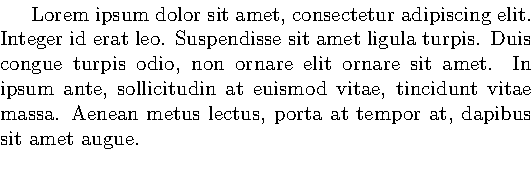
\includegraphics[width=\linewidth,height=0.5\textheight,keepaspectratio]{assets/singleParagraph2.pdf}
			\end{column}
		\end{columns}
		\pause
		\begin{columns}
			\begin{column}{0.5\textwidth}
				\useblock{paragraphs2}
			\end{column}
			\begin{column}{0.5\textwidth}
				\only<3->{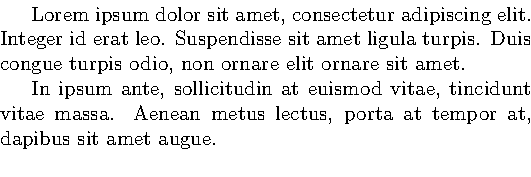
\includegraphics[width=\linewidth,height=0.5\textheight,keepaspectratio]{assets/doubleParagraph.pdf}}
			\end{column}
		\end{columns}
		\pause
	\end{frame}

	\begin{saveblock}{paragraphs}
		\begin{highlightblock}[linewidth=0.5\textwidth,gobble=12]
			\noindent Lorem ipsum dolor
			sit amet, ... ornare sit
			amet.
			
			In ipsum ante, sollicitudin
			... sit amet augue.
		\end{highlightblock}
	\end{saveblock}

	\addtorecentlist{\textbf{\textbackslash noindent}}

	\begin{frame}
		\frametitle{Alinea's en regels}
		
		\begin{columns}
			\begin{column}{0.5\textwidth}
				\useblock{paragraphs}
			\end{column}
			\begin{column}{0.5\textwidth}
				\only<2->{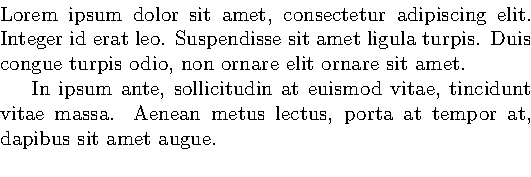
\includegraphics[width=\linewidth,height=0.5\textheight,keepaspectratio]{assets/paragraphsNoIndent.pdf}}
			\end{column}
		\end{columns}
	\end{frame}

	\begin{saveblock}{paragraphs}
		\begin{highlightblock}[linewidth=0.5\textwidth,gobble=12]
			...
			\usepackage{parskip}
			\begin{document}			
			Lorem ipsum dolor sit amet,
			... ornare sit amet.
			
			In ipsum ante, sollicitudin
			... sit amet augue.
			\end{document}
		\end{highlightblock}
	\end{saveblock}

	\addtorecentlist{\textbf{parskip}}

	\begin{frame}
		\frametitle{Alinea's en regels}
		
		\begin{columns}
			\begin{column}{0.5\textwidth}
				\useblock{paragraphs}
			\end{column}
			\begin{column}{0.5\textwidth}
				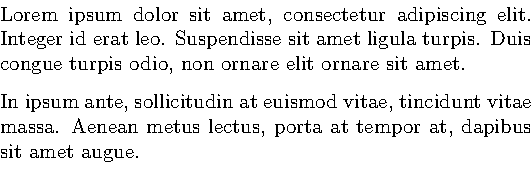
\includegraphics[width=\linewidth,height=0.8\textheight,keepaspectratio]{assets/paragraphsParskip.pdf}
				
%				\only<2->{\scriptsize{Zonder parskip:}
%				
%				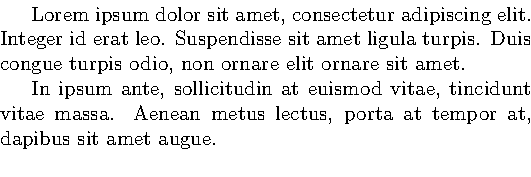
\includegraphics[width=\linewidth,height=0.5\textheight,keepaspectratio]{assets/doubleParagraph.pdf}}
			\end{column}
		\end{columns}
	\end{frame}


	\begin{saveblock}{paragraphs}
		\begin{highlightblock}[linewidth=0.5\textwidth,gobble=12]
			Lorem ipsum dolor sit amet,
			... ornare sit amet.
			\vspace{1cm}
			
			In ipsum ante, sollicitudin
			... sit amet augue.
		\end{highlightblock}
	\end{saveblock}

	\addtorecentlist{\textbf{\textbackslash vspace}}
	
	\begin{frame}
		\frametitle{Alinea's en regels}
		
		\begin{columns}
			\begin{column}{0.5\textwidth}
				\useblock{paragraphs}
			\end{column}
			\begin{column}{0.5\textwidth}
				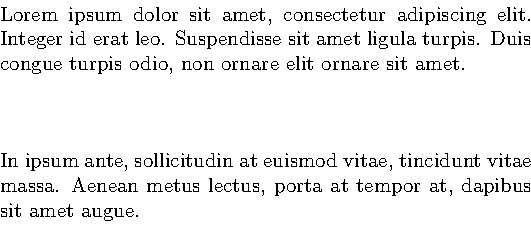
\includegraphics[width=\linewidth,height=0.8\textheight,keepaspectratio]{assets/paragraphsVspace.pdf}
			\end{column}
		\end{columns}
	
		\par\tiny{(Steeds parskip vanaf nu)}
	
	\end{frame}


	
%	\begin{frame}
%		\frametitle{Alinea's en regels}
%		
%
%	\end{frame}
	
	%\begin{frame}
	%	\frametitle{Teksteffecten}
	%	
	%	\hll|\{\\fontsize\{50\}\{60\}\\selectfont Hi!\}|
	%	\par\addvspace{10px}
	%	
	%	{\centering {\fontsize{150}{130}\selectfont Hi!}}
	%\end{frame}
	
	\addtorecentlist{\textbf{enumerate}}
	
	\begin{saveblock}{list}
		\begin{highlightblock}[linewidth=0.5\textwidth,gobble=12]
			Dit zijn de ingredi~\"e~nten:
			\begin{enumerate}
				\item Wortels				
				\item Uien
				
				Lipsum dolor sit amet.
				\item Aardappelen
			\end{enumerate}
		\end{highlightblock}
	\end{saveblock}
	
	\begin{frame}
		\frametitle{Lijsten}
		
		\begin{columns}
			\begin{column}{0.5\textwidth}
				\useblock{list}
			\end{column}
			\begin{column}{0.5\textwidth}
				%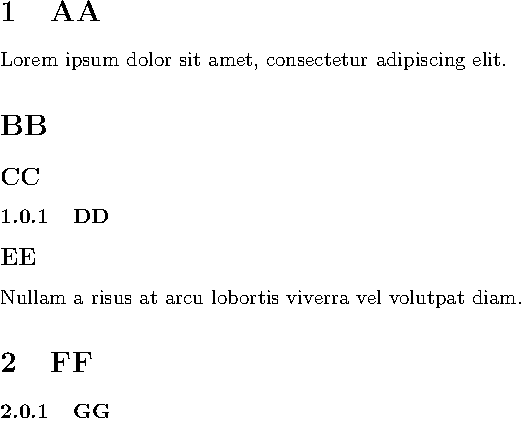
\includegraphics[width=\linewidth,height=0.8\textheight,keepaspectratio]{assets/partialNumberedStars.pdf}
				Dit zijn de ingrediënten:
				\begin{enumerate}
					\item Wortels
					\item Uien
					
					Lipsum dolor sit amet.
					\item Aardappelen
				\end{enumerate}
			\end{column}
		\end{columns}
	\end{frame}

	\begin{saveblock}{list}
		\begin{highlightblock}[linewidth=0.5\textwidth,gobble=12]
			Dit zijn de ingredi~\"e~nten:
			\begin{enumerate}
				\item Wortels
				\begin{enumerate}
					\item Kopen
					\item Raspen
					\item Fijnsnijden
				\end{enumerate}			
				\item Uien
				
				Lipsum dolor sit amet.
				\item Aardappelen
			\end{enumerate}
		\end{highlightblock}
	\end{saveblock}
	
	\begin{frame}
		\frametitle{Lijsten}
		
		\begin{columns}
			\begin{column}{0.5\textwidth}
				\useblock{list}
			\end{column}
			\begin{column}{0.5\textwidth}
				%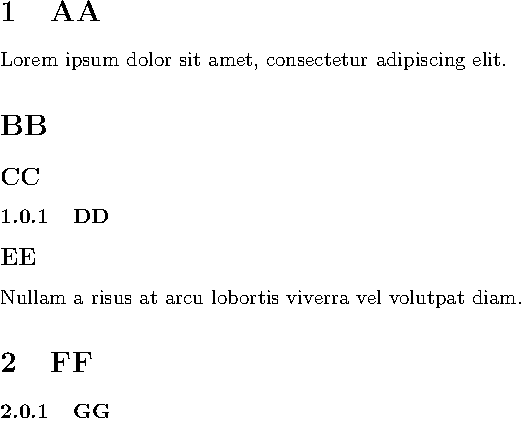
\includegraphics[width=\linewidth,height=0.8\textheight,keepaspectratio]{assets/partialNumberedStars.pdf}
				Dit zijn de ingrediënten:
				\begin{enumerate}
					\item Wortels
					\begin{enumerate}
						\item Kopen
						\item Raspen
						\item Fijnsnijden
					\end{enumerate}
					\item Uien
					
					Lipsum dolor sit amet.
					\item Aardappelen
				\end{enumerate}
			\end{column}
		\end{columns}
	\end{frame}

	\addtorecentlist{\textbf{itemize}}

	\begin{saveblock}{list}
		\begin{highlightblock}[linewidth=0.5\textwidth,gobble=12]
			Dit zijn de ingredi~\"e~nten:
			\begin{itemize}
				\item Wortels
				\begin{enumerate}
					\item Kopen
					\item Raspen
					\item Fijnsnijden
				\end{enumerate}			
				\item Uien
				
				Lipsum dolor sit amet.
				\item Aardappelen
			\end{itemize}
		\end{highlightblock}
	\end{saveblock}
	
	\begin{frame}
		\frametitle{Lijsten}
		
		\begin{columns}
			\begin{column}{0.5\textwidth}
				\useblock{list}
			\end{column}
			\begin{column}{0.5\textwidth}
				%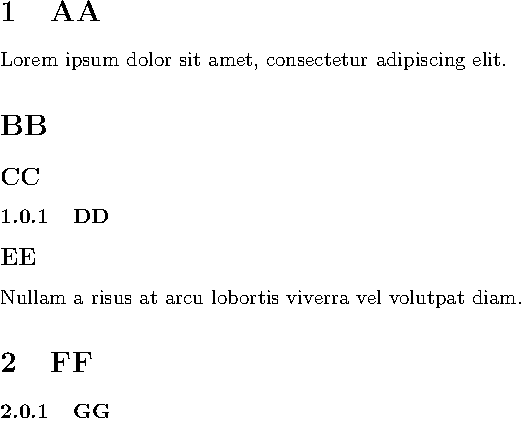
\includegraphics[width=\linewidth,height=0.8\textheight,keepaspectratio]{assets/partialNumberedStars.pdf}
				Dit zijn de ingrediënten:
				\begin{itemize}
					\item Wortels
					\begin{enumerate}
						\item Kopen
						\item Raspen
						\item Fijnsnijden
					\end{enumerate}
					\item Uien
					
					Lipsum dolor sit amet.
					\item Aardappelen
				\end{itemize}
			\end{column}
		\end{columns}
	\end{frame}

	\begin{saveblock}{list}
		\begin{highlightblock}[linewidth=0.5\textwidth,gobble=12]
			Dit zijn de ingredi~\"e~nten:
			\begin{itemize}
				\item Wortels
				\begin{itemize}
					\item Kopen
					\item Raspen
					\item Fijnsnijden
				\end{itemize}			
				\item Uien
				
				Lipsum dolor sit amet.
				\item Aardappelen
			\end{itemize}
		\end{highlightblock}
	\end{saveblock}
	
	\begin{frame}
		\frametitle{Lijsten}
		
		\begin{columns}
			\begin{column}{0.5\textwidth}
				\useblock{list}
			\end{column}
			\begin{column}{0.5\textwidth}
				%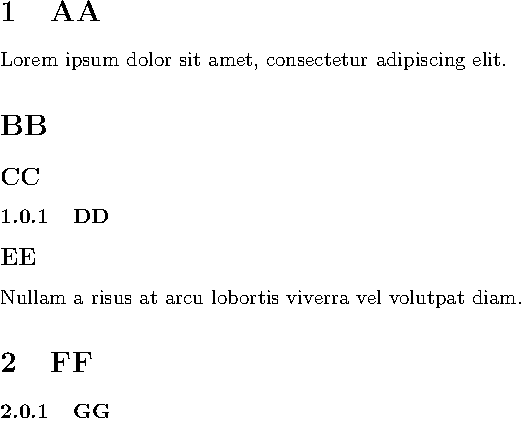
\includegraphics[width=\linewidth,height=0.8\textheight,keepaspectratio]{assets/partialNumberedStars.pdf}				
				Dit zijn de ingrediënten:
				\begin{itemize}
					\item Wortels
					\begin{itemize}
						\item[\textbullet] Kopen
						\item[\textbullet] Raspen
						\item[\textbullet] Fijnsnijden
					\end{itemize}
					\item Uien
					
					Lipsum dolor sit amet.
					\item Aardappelen
				\end{itemize}
			\end{column}
		\end{columns}
	\end{frame}

	\begin{saveblock}{specSymb}
		\begin{highlightblock}[linewidth=0.5\textwidth,gobble=12]
			\textbf{Hey},
			\textbackslash textbf,
			% Opmerking
			Wel 90% {van} de
			'respondenten'
			
			Wel 90\% {van} de
			~\textasciigrave~respondenten'
			
			Daarom \&, \$, \{van\},
			\textasciitilde,
			\textasciigrave respondenten
			'
		\end{highlightblock}
	\end{saveblock}

	\addtorecentlist{\textbf{speciale tekens}}

	\begin{frame}
		\frametitle{Speciale tekens}
		
		\begin{columns}
			\begin{column}{0.5\textwidth}
				\useblock{specSymb}
			\end{column}
			\begin{column}{0.5\textwidth}
				\textbf{Hey},
				\textbackslash textbf,
				% Opmerking
				Wel 90% {van} de
				'respondenten'
				
				Wel 90\% {van} de
				`respondenten'
				
				Daarom \&, \$, \{van\},
				\textasciitilde,
				\textasciigrave respondenten
				'
			\end{column}
		\end{columns}
		
	\end{frame}

%	\begin{frame}
%		\begin{enumerate}
%			\item Speciale tekens
%			\item Lijsten
%			\item Pagina layout
%			\item Inhoudstafel
%		\end{enumerate}
%	\end{frame}
\end{document}
